\section{Parametrisierte Algorithmen}

\begin{takeaway}
    \item Parametrisierter Algorithmus, fpt
    \item Standard-Parametrisierung
    \item Kernbildung
    \item (Sichere) Datenreduktionsregel
    \item Kronenzerlegung
\end{takeaway}

\paragraph{Idee}
Verallgemeinerung von pseudopolynomiellen Algorithmen:
Laufzeit hängt von der Eingabegrösse nur polynomiell ab, aber darf extrem gross werden in der Grösse eines Parameters.
Partitionierung in Problemklassen entlang des Parameters.

\paragraph{Parametrisierung}
Sei $U$ ein Entscheidungsproblem, $L$ die Sprache der Eingaben.
$\Par: L \mapsto \N$ ist eine \emph{Parametrisierung} von $U$ falls gilt:
\begin{enumerate}[label=(\roman*)]
    \item $\Par$ ist in Polynomzeit berechenbar
    \item Für unendlich viele $k \in \N$ ist die Parameter-$k$-Menge für $U$
    $$ Set_U(k) := \{ I \in L \st \Par(I) = k \} $$ unendlich.
    Dies stellt sich dass $\Par$ nichttrivial ist, z.B. nicht etwa $\Par(I) = |I|$.
    In anderen Worten, für jeden Parameterwert soll es beliebig viele Probleminstanzen geben.
\end{enumerate}
Ein Algorithmus $\A$ heisst \emph{$\Par$-paremetrisierter Polynomzeit-Algorithmus} für $U$ falls gilt:
\begin{enumerate}[label=(\roman*)]
    \item $\A$ löst $U$
    \item $ \exists \text{ Polynom } p \; \exists \text{ (berechenbare) Funktion } f : \N \mapsto \N$
    so dass $\forall I \in L$:
    $$\Time_\A(I) \leq f \big( \Par(I) \big) \cdot p(|I|) $$
\end{enumerate}
Dann heisst $U$ \emph{fixed-parameter-tractable bezüglich $\Par$}.
$\A$ heisst auch \emph{fpt-Algorithmus für $U$ bezüglich $\Par$} und läuft in fpt-Zeit.

\underline{Beispiel:}
Sei $U$ ein Zahlproblem und sei $Val(I) := \max \{ |x_i| \}$.
Es gilt $Max-Int(I) \leq 2^{Val(I)}$ und ist $Val$ eine Parametrisierung von $U$.

\paragraph{Ansätze}
Die \emph{Standard-Parametrisierung} wählt als Parameter die Grösse der gewünschten Lösung (z.B. Grösse des VCs).
Die \emph{Strukturelle Parametrisierung} wählt eine bestimmte Eigenschaft der Eingabe (z.B. maximaler Knotengrad).
Andere Ansätze betrachten wir im Folgenden.


\subsection{Kernbildung}

\paragraph{Idee}
Polynomielles Preprocessing, Datenreduktion, um die Instanz auf einen \emph{Kern} zu verkleinern,
der in seiner Grösse nur noch vom Parameter abhängt.
Diesen Kern dann mit bekannten Algorithmen (oder brute force) lösen.

\paragraph{Kernbildung (kernelisation)}
Sei $(U, \Par)$ ein parametrisiertes Entscheidungsproblem, $L$ die Sprache der JA-Instanzen von $U$.
Ein \emph{Kernbildungs-Algorithmus} für $(U, \Par)$ ist ein Polynomzeit-Algorithmus $\A$ der jede Eingabe $(I, k)$
in eine neue Eingabe $(I', k')$ (den \emph{Kern (kernel)}) transformiert so dass:
\begin{enumerate}[label=(\roman*)]
    \item $ I \in L \iff I' \in L $ (Korrektheit)
    \item $ |I'| + k' \leq g(k) $ für $g : \N \mapsto \N$ (neue Grösse nur abhängig vom alten Parameterwert $k$)
\end{enumerate}

Eine \emph{Reduktionsregel} von $\A$ heisst \emph{sicher}, wenn sie (i) erfüllt.

\paragraph{Beispiel: VCP} \mbox{} \\
\underline{Reduktionsregel:}
Sei $S \subseteq V$ ein VC von $G$ so dass $|S| \leq k$. Dann enthält $S$ alle Knoten mit $\deg_G(v) > k$ (warum?).
Dann gilt für ein solches $v$:
$$ (G, k) \in VCP \iff (G-\{v\}, k-1) \in VCP $$
Zusätzlich entferne alle isolierten Knoten mit $\deg_G(v) = 0$ (sie decken keine Kanten ab).

Zu zeigen: wenn die Regel nicht mehr anwendbar ist, dann hat der verbleibende Graph $G'$ entweder kein vertex cover,
oder aber er ist ``klein genug'' (nur noch anhängig von $k$), also ein Kern.

\underline{Beobachtung:}
Sei $G$ ein Graph ohne isolierten Knoten, mit einem vertex cover der Grösse $m$ und mit $\max \deg_G(v) \leq k$.
Dann gilt $|V| \leq m \cdot (k+1)$ (warum?).%
\footnote{Falls $|V| > k \cdot (k+1)$, dann wir wissen dass $ I \notin L$ und können NEIN ausgeben.}

\underline{Theorem:}
Diese Reduktionsregeln berechnen einen Kern der Grösse $\bigO (k^2)$ in Zeit $\bigO (k \cdot n)$.

\underline{Parametrisierter Algorithmus:}
Berechne einen Kern $(G', k')$. Wenn der Kern zu gross ist, geben NEIN aus.
Andernfalls prüfe durch vollständige Suche ob ein VC mit $|S'| \leq k'$ existiert.

\underline{Theorem:}
Dies ist ein fpt-Algorithmus bzgl. der Standard-Parametrisierung. Die Laufzeit beträgt
$\bigO (k \cdot n + k^{2k+2}) \subseteq \bigO (k^{2k+2} \cdot n)$.

\paragraph{Theorem}
Sei $(U, \Par)$ ein parametrisiertes Entscheidungsproblem. \\
Ein fpt-Algorithmus für $(U, \Par)$ existiert $\iff$ Ein Kernbildungsalgorithmus für $(U, \Par)$ existiert.

\paragraph{Edge Clique Cover Problem ECCP} \mbox{} \\
Eingabe: ungerichteter Graph $G=(V,E)$, $k \leq \N$ \\
Ausgabe: JA falls $k$ Cliquen $C_1, \dots, C_k$ existieren, so dass $E = \bigcup_{i=1}^k E(C_i)$, sonst NEIN.

\underline{Reduktionsregeln:}
\begin{enumerate}[label=(\roman*)]
    \item $(G, k) \xrightarrow{\text{isolierter Knoten } u} (G-\{ u \}, k)$
    \item $(G, k) \xrightarrow{\text{isolierte Kante } e=\{u,v\} } (G-\{ u,v \}, k-1)$
    \item $(G, k) \xrightarrow{\{u,v\} \in E \text{ s.t. } \{u,v\} \subsetneq N[u] = N[v] } (G-\{ u \}, k)$ \\
    $N[u]$ ist die \emph{geschlossene Nachbarschaft} von $u$, also alle benachbarten Knoten und $u$ selbst.
\end{enumerate}

\underline{Theorem:} Das ECCP hat einen Kern mit $\leq 2^k$ Knoten.


\subsubsection{Kronenzerlegung}

Ziel: statt einem quadratischen Kern suchen wir einen linearen Kern für das VCP. \\
Bisher genutzte Strukturen zur Reduktion: hoher Knotengrad, gleiche geschlossene Nachbarschaft.

\paragraph{Kronenzerlegung (crown decomposition)}
Die \emph{Kronenzerlegung} von $G=(V,E)$ ist eine Partitionierung $V = C \cup H \cup B$ so dass:
\begin{enumerate}[label=(\roman*)]
    \item $C \neq \emptyset$ ist ein independent set in $G$
    \item $N(C) = H$ (keine Kanten zwischen $C$ und $B$)
    \item Die Kanten zwischen $C$ und $H$ enthalten ein Matching $M$ mit $|M| = |H|$ ($M$ \emph{saturiert} $H$).
\end{enumerate}

\begin{figure}[h]
    \centering
	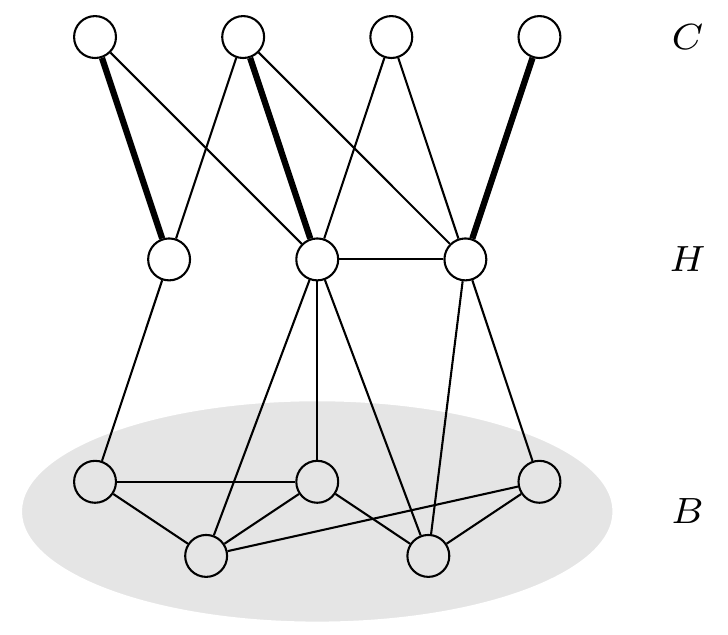
\includegraphics[scale=0.4]{images/crown-decomp.png}
    \caption{Kronenzerlegung: crown, head, body (Quelle: Vorlesung)}
    \label{fig:crown-decomp}
\end{figure}

\paragraph{Satz von König}
Sei $G$ ein ungerichteter bipartiter Graph, sei $M$ ein Matching maximaler Kardinalität,
sei $S$ ein vertex cover minimaler Kardinalität.
Dann gilt $|M| = |S|$.

\underline{Theorem:} $M$ und $S$ können in Polynomzeit berechnet werden.

\paragraph{Lemma}
Sei $G$ ungerichtet, ohne isolierte Knoten, mit $|V| \geq 3k+1$.
Dann existiert ein Polynomzeitalgorithmus der
\begin{enumerate}[label=(\roman*)]
    \item entweder eine Kronenzerlegung berechnet
    \item oder ein Matching $M$ mit $|M| \geq k+1$ findet.
\end{enumerate}
Beweis siehe Buch, Kapitel 6.2, Seite 145f.

\paragraph{Reduktion für VCP} \mbox{} \\
\underline{Lemma:}
Sei $G$ ein Graph mit Kronenzerlegung $V = C \cup H \cup B$ und sei $k \in \N$. Dann gilt: \\
$G$ hat ein vertex cover der Grösse $k$ $\iff$ $G - (C \cup H)$ hat ein vertex cover der Grösse $k - |H|$.

\underline{Theorem:} Ein Kernbildungsalgorithmus mit obiger Reduktionsregel findet einen Kern mit $\leq 3k$ Knoten.


\subsection{Suchbäume}


\subsection{Iterative Kompression}


